\chapter{Evaluation}
\label{cha:evaluation}

\quad This chapter describes the practical aspects of the experiments and its results. Initially, the study focused on understanding the theoretical behavior of the methods and the capabilities of CL. Once the requirements stood clear, the focus shifted to the physical project, where with the help of tools \cite{SDK} and as explained in \ref{sec:creation_of_project}, it was possible to understand where to collect the information needed for the CL development. The workflow for the generation of the base template starts with the design of a base model. Then is the training of the classification model based on a Mnist dataset \cite{deng2012mnist} using PyTorch functions adapted to the Maxim tools \cite{ai8x-training}. Afterward is the loading of the network on the embedded device, which is accomplished by the network loader \cite{ai8x-synthesis}. Now is time to collect the new dataset \cite{cohen2017emnist} needed for the CL system to work.

\section{Dataset Collection}
\label{sec:dataset_collection}

\quad This study uses the Emnist dataset. The Emnist dataset is a voluminous publicly available collection of images of hand-written digits having a size of 28 x 28 pixels, specifically the letters collection. It is composed of 145,600 characters balanced in 26 classes. Figure \ref{emnist_example} shows examples of Emnist images. For this study, Python scripts are used to collect the chosen letters 'A' and 'a' from the original dataset. A first conversion is needed from the dataset collection to a NumPy pickle then the synthesizer alters the pickles into samples for the MCU. This transformation is needed because the embedded device uses a characteristic input. After that, another script creates a long array of sample input ready to be used. Due to space constraints, exclusively 40 training samples could be loaded into the memory on the device.  

\begin{figure}[!ht]
\centerline{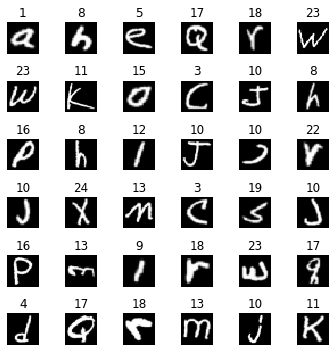
\psfig{file=Images/emnist_examples.png,width=0.6\textwidth}}
\caption{Example of images from Emnist dataset}
\label{emnist_example}
\end{figure}

\section{Network Model}
\label{sec:network_model}

\quad Convolutional Neural Network (CNN) model is the architecture used in this image classification application. Computer vision uses CNN models for the elaboration of images. Its main feature is the presence of convolutional layers for feature extraction. This type of structure allows the ML model to perform initially a feature extraction over the image and to flatten the output matrix to an array. Following is the NN layer for the classification. Figure \ref{input_output_model} represent the structure of the model. The frozen model contains four convolutional layers followed by the ReLU activation function \ref{relu}. The last 3 layers of the frozen model are Max pooled and Avg pooled. The fully connected layer is used to elaborate the array and later feed the data to the classification layer, where the Softmax activation function is used to produce the probability of each class. 

\begin{figure}[!ht]
\centerline{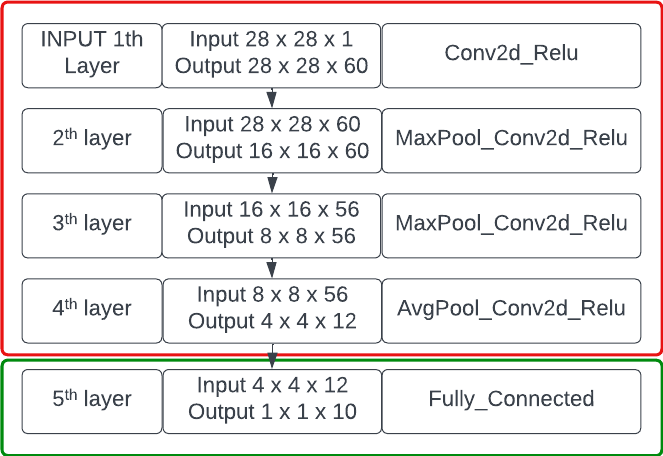
\psfig{file=Images/Input_output_model.png,width=0.6\textwidth}}
\caption{Description of the model. Structure and input-output size. Frozen model in red, and CL layer in green}
\label{input_output_model}
\end{figure}

\section{Model Training}
\label{sec:model_training}

\quad It was possible to obtain the base model through the tools given by Maxim. As said before, the base model is the Mnist network. During the training, it was possible to monitor the progress and performance of the model. This phase was crucial to designing the best-performing network. Figure \ref{training_results} the results of the training over epochs.

\begin{figure}[!ht]
\centering
     \begin{subfigure}[b]{0.4\textwidth}
         \centering
         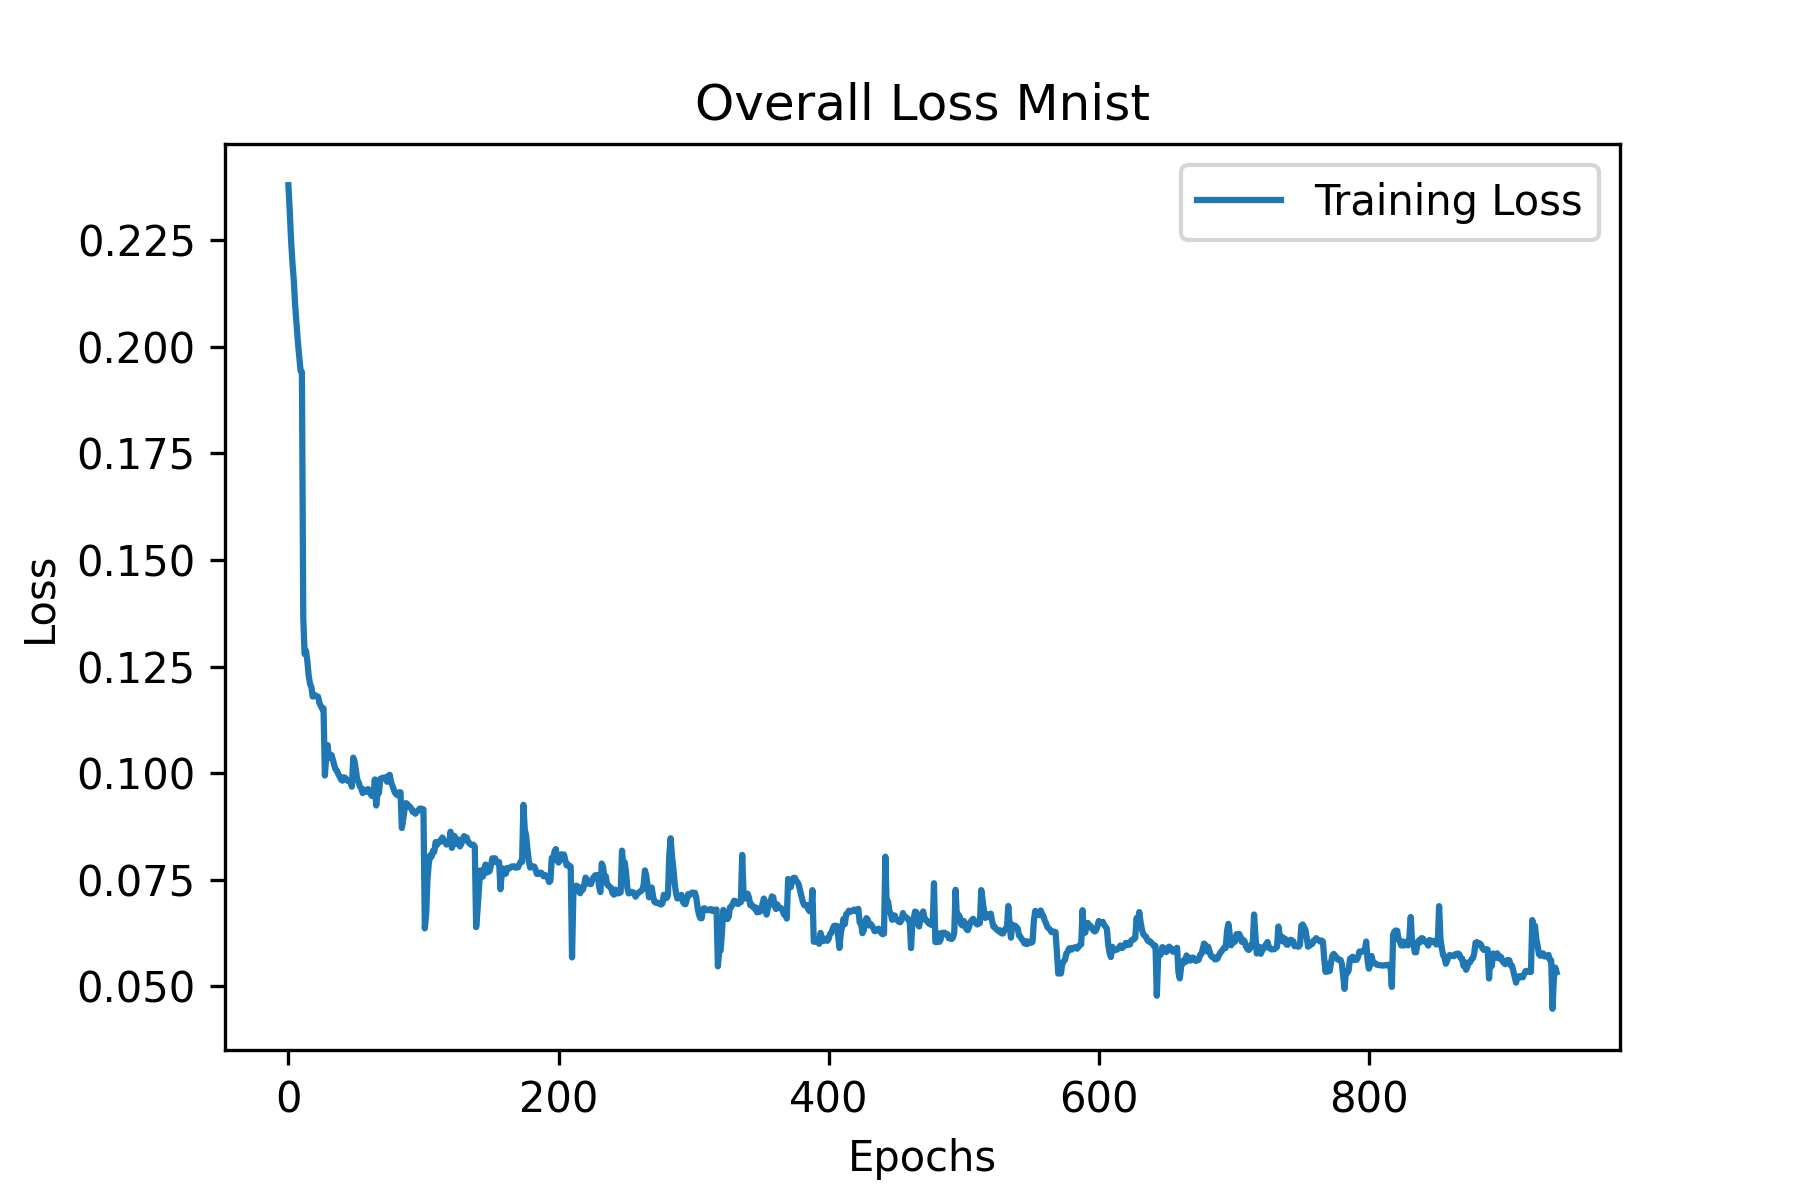
\includegraphics[width=\textwidth]{Images/plot_training_loss_mnist.png}
         \caption{Overall loss of training over time.}
         \label{fig:training_loss}
     \end{subfigure}
     \hfill
     \begin{subfigure}[b]{0.4\textwidth}
         \centering
         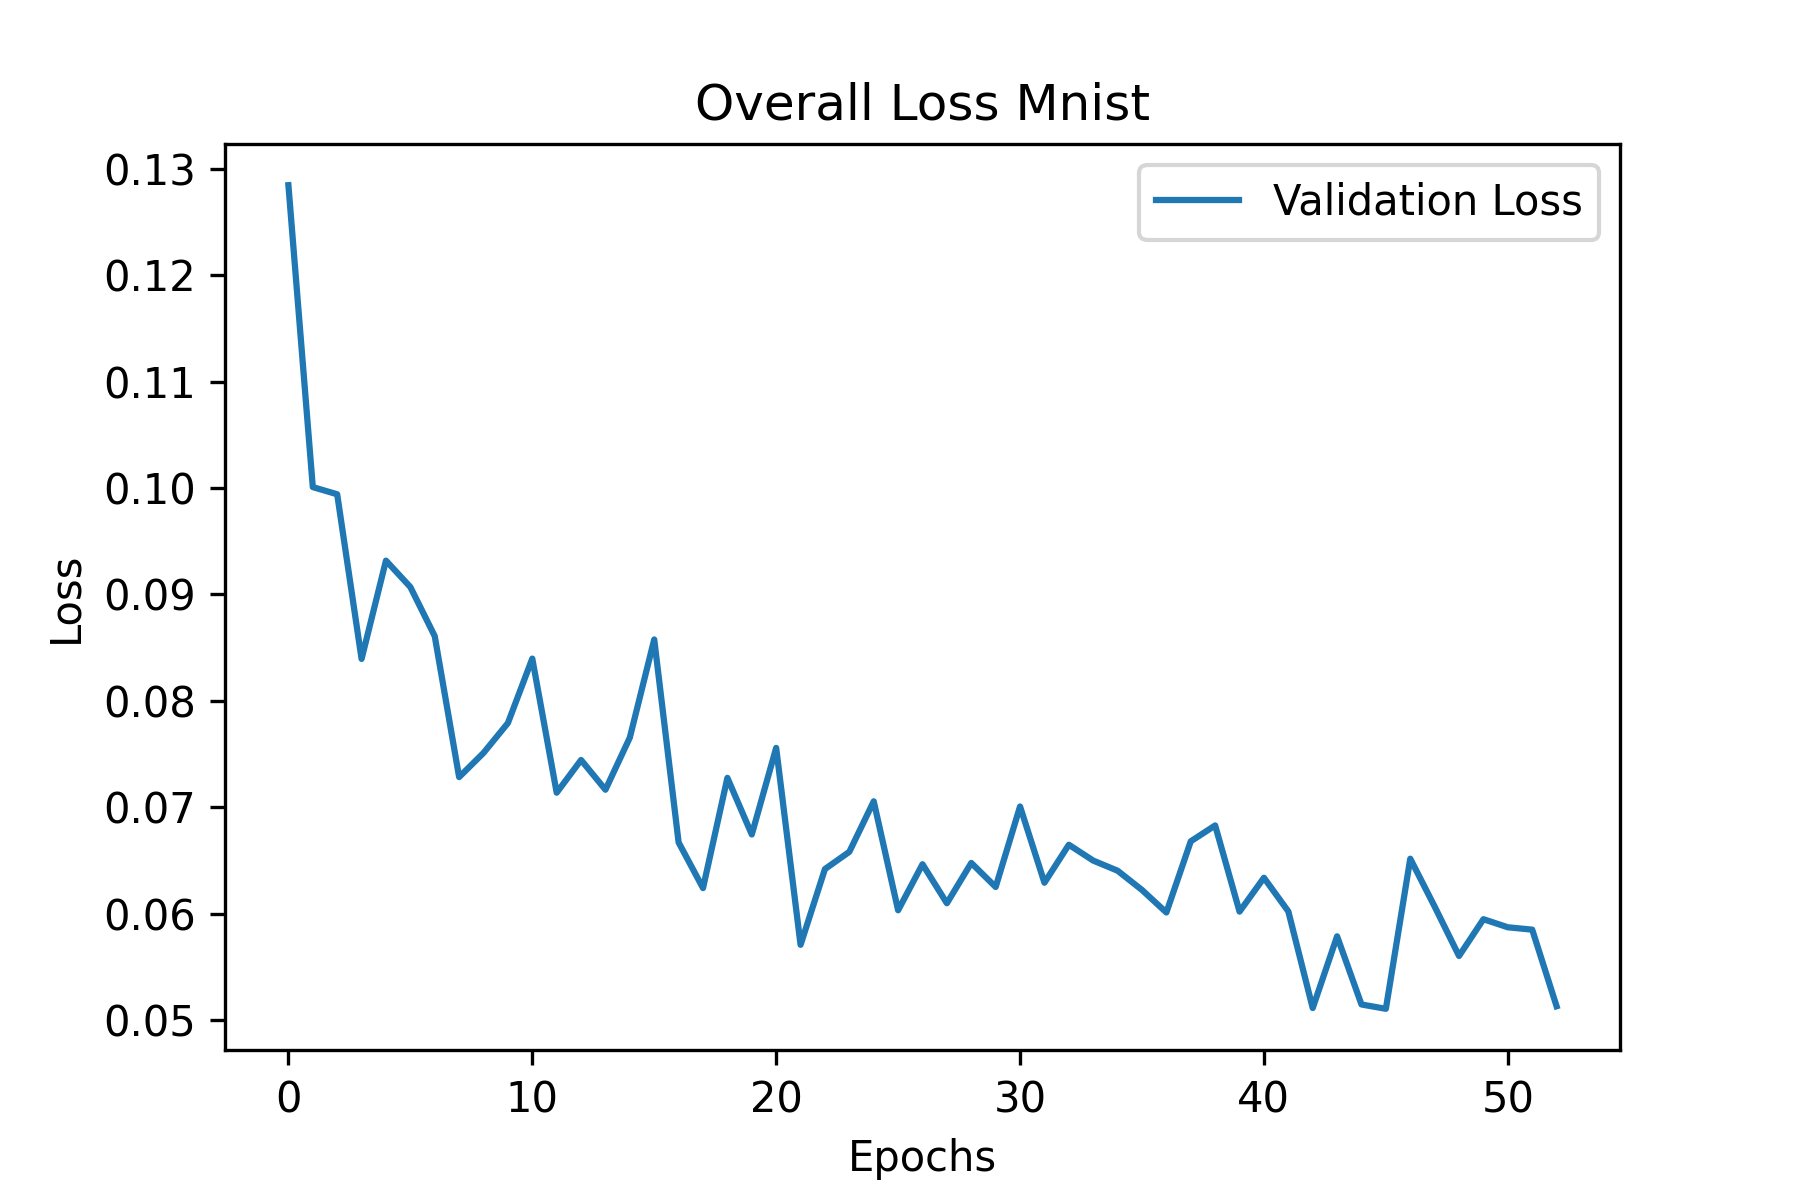
\includegraphics[width=\textwidth]{Images/plot_validation_loss_mnist.png}
         \caption{Overall loss of validation over time.}
         \label{fig:validation_loss}
     \end{subfigure}
     \hfill
     \begin{subfigure}[b]{0.4\textwidth}
         \centering
         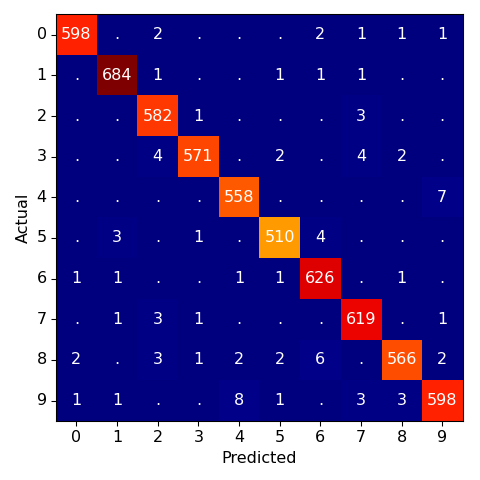
\includegraphics[width=\textwidth]{Images/plot_mnist_confusion_matrix.png}
         \caption{Confusion matrix.}
         \label{fig:confusion_matrix}
     \end{subfigure}
        \caption{Training results of Mnist model training taken with Tensorflow}
        \label{training_results}
\end{figure}

\section{Frozen Model}
\label{sec:frozen_model}

\quad In the embedded device field, memory and speed are key features. Designing the model considering the memory constraint is a fundamental step. Because of this, the model is a tiny example of a Neural Network, composed of 5 layers. In the application, the frozen model is composed of 4 layers, which are used for the feature extraction. Since the images of the two datasets have similar features, this project uses the same frozen model for the two different images. The comparison plot can be seen in \ref{comparison_frozen_model}. 

\begin{figure}[!ht]
\centerline{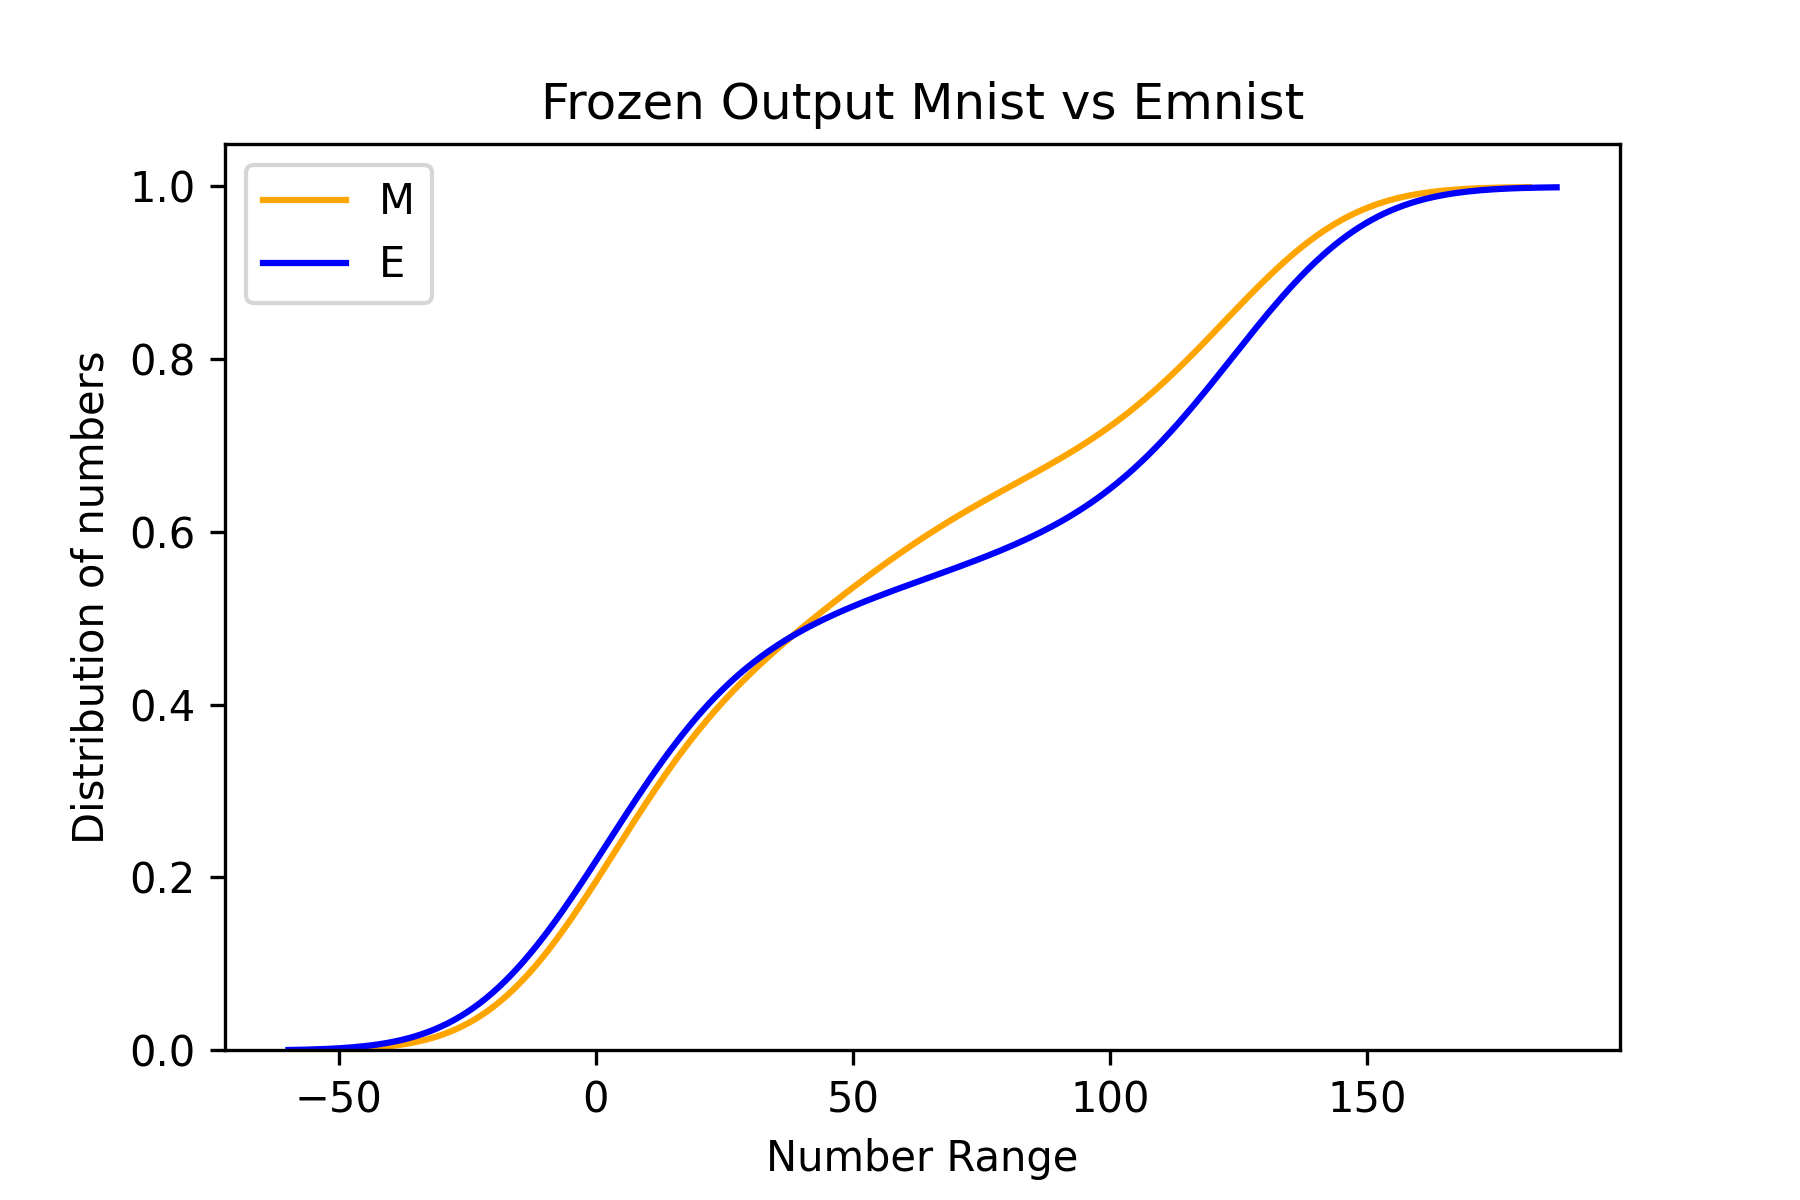
\psfig{file=Images/plot_frozen_model_emnist_mnist.png,width=0.8\textwidth}}
\caption{Comparison of output of feature extractions Mnist vs Emnist}
\label{comparison_frozen_model}
\end{figure}

\section{Max78000 setup}
\label{sec:application_setup}

\quad This section describes the setup needed to run the application correctly and explains each step. First, to deploy the code is necessary to configure the computer as explained in \cite{SDK}, the tools used are OpenOCD and Arm-gdb which allows a connection to the board permitting the flashing of codes. The dataset, model, final layer, and system can all be deployed on the MCU once they are all ready.  Initially, the code set up the board parameters, such as the clock source and the debugger, then it enables the CNN accelerator clock and starts a loop. Each loop is composed like this: first, there is the initialization and the loading of weights biases and inputs, followed by the configuration and inferences of the CNN, during which the output of the frozen layer is captured. Following is the computation of the channel's outputs, which will be used to calculate the update values. In the end is the back-propagation phase, which updates neuron weights and biases according to the Softmax function. When the loop ends, the code computes complete inferences on training and testing samples to correctly classify the system accuracy. Additionally, an inference on a Mnist digit is computed to check if during the CL training the catastrophic forgetting happened.


\section{Experimental Results}
\label{cha:experimental_results}

\quad The next sections describe and discuss all the results of the experiment performed. The system is developed in the MCU, but on the other hand, the experiment's results have been docketed by the MCU itself or an external device. Time and energy consumption are measured with X-NUCLEO-LPM01A \cite{nucleo}. The test has been carried out in a supervised environment, where the sample data are established a priori. The input samples handled are all 'A's taken from the EMNIST dataset. In this way, it was possible to make an ideal model classification. 

\section{Continual Learning on Max78000 Microcontroller}
\label{sec:image_classification}

\quad The aim is to replace the weights and biases of the neuron responsible for recognizing class 0. Specifically, previously this neuron had the task of identifying the digit 0, then because of continual learning, it can recognize the letter A. Due to memory constraints a total of 40 samples have been used to fulfill the training. THe table represented in Figure \ref{time_inferences} shows an overview of times for the frozen model inference and the CL system. In this case the average inference time of the frozen model includes the weights and biases loading, and the initialization and configuration of the CNN accelerator. Different clock sources are applied, and in every case, is preserved the same ratio. Figure \ref{time_single_layer} displays the time that each layer take to perform inference. The clock of the CNN accelerator has a maximum speed of 50 MHz. The hardware-based accelerator computes inferences in a short time. 

\begin{figure}[!ht]
\centerline{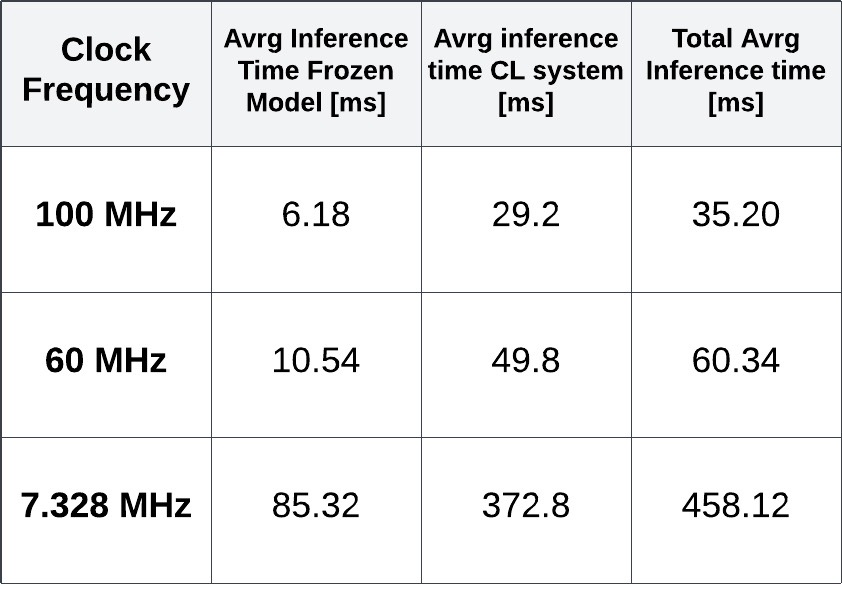
\psfig{file=Images/time_inference_cl_table.png,width=0.8\textwidth}}
\caption{Table comparing the overall time of initialization and inference of frozen model and CL layer with different clock sources.}
\label{time_inferences}
\end{figure}

\begin{figure}[htbp]
\centerline{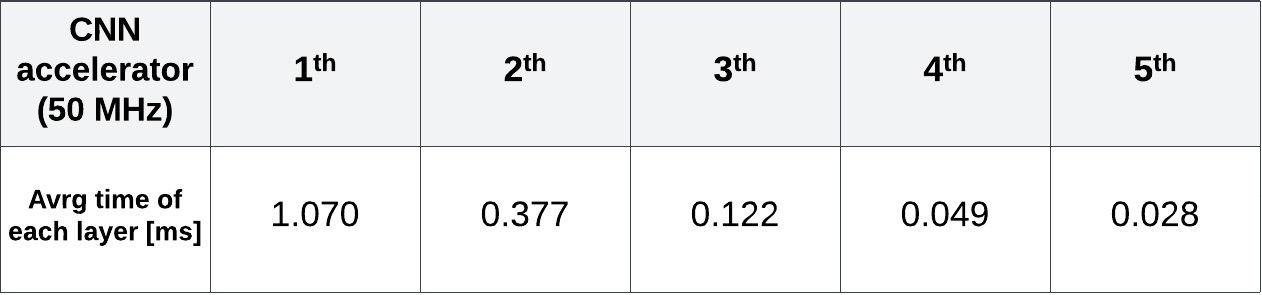
\psfig{file=Images/time_single_layer_inference_cnn.png,width=0.8\textwidth}}
\caption{Table showing time inferences of each layer inside the CNN accelerator.}
\label{time_single_layer}
\end{figure}

\singlespacing

\quad Figure \ref{time_backpropagations_iterations} illustrates two distributions of time needed to apply the back-propagation. The first plot shows the time distribution of 100 iterations, figuring the weights update does not occur at each loop, but it happens just when an update is needed. According to the algorithm, the update occurs just when a classification turns out wrong. It is possible to state that, as seen in the \ref{fig:time_1000_iterations} plot, after some iterations, the update stops to happens because the system adjusted the weights to recognize the new class.

\begin{figure}[!ht]
\centering
     \begin{subfigure}[b]{0.4\textwidth}
         \centering
         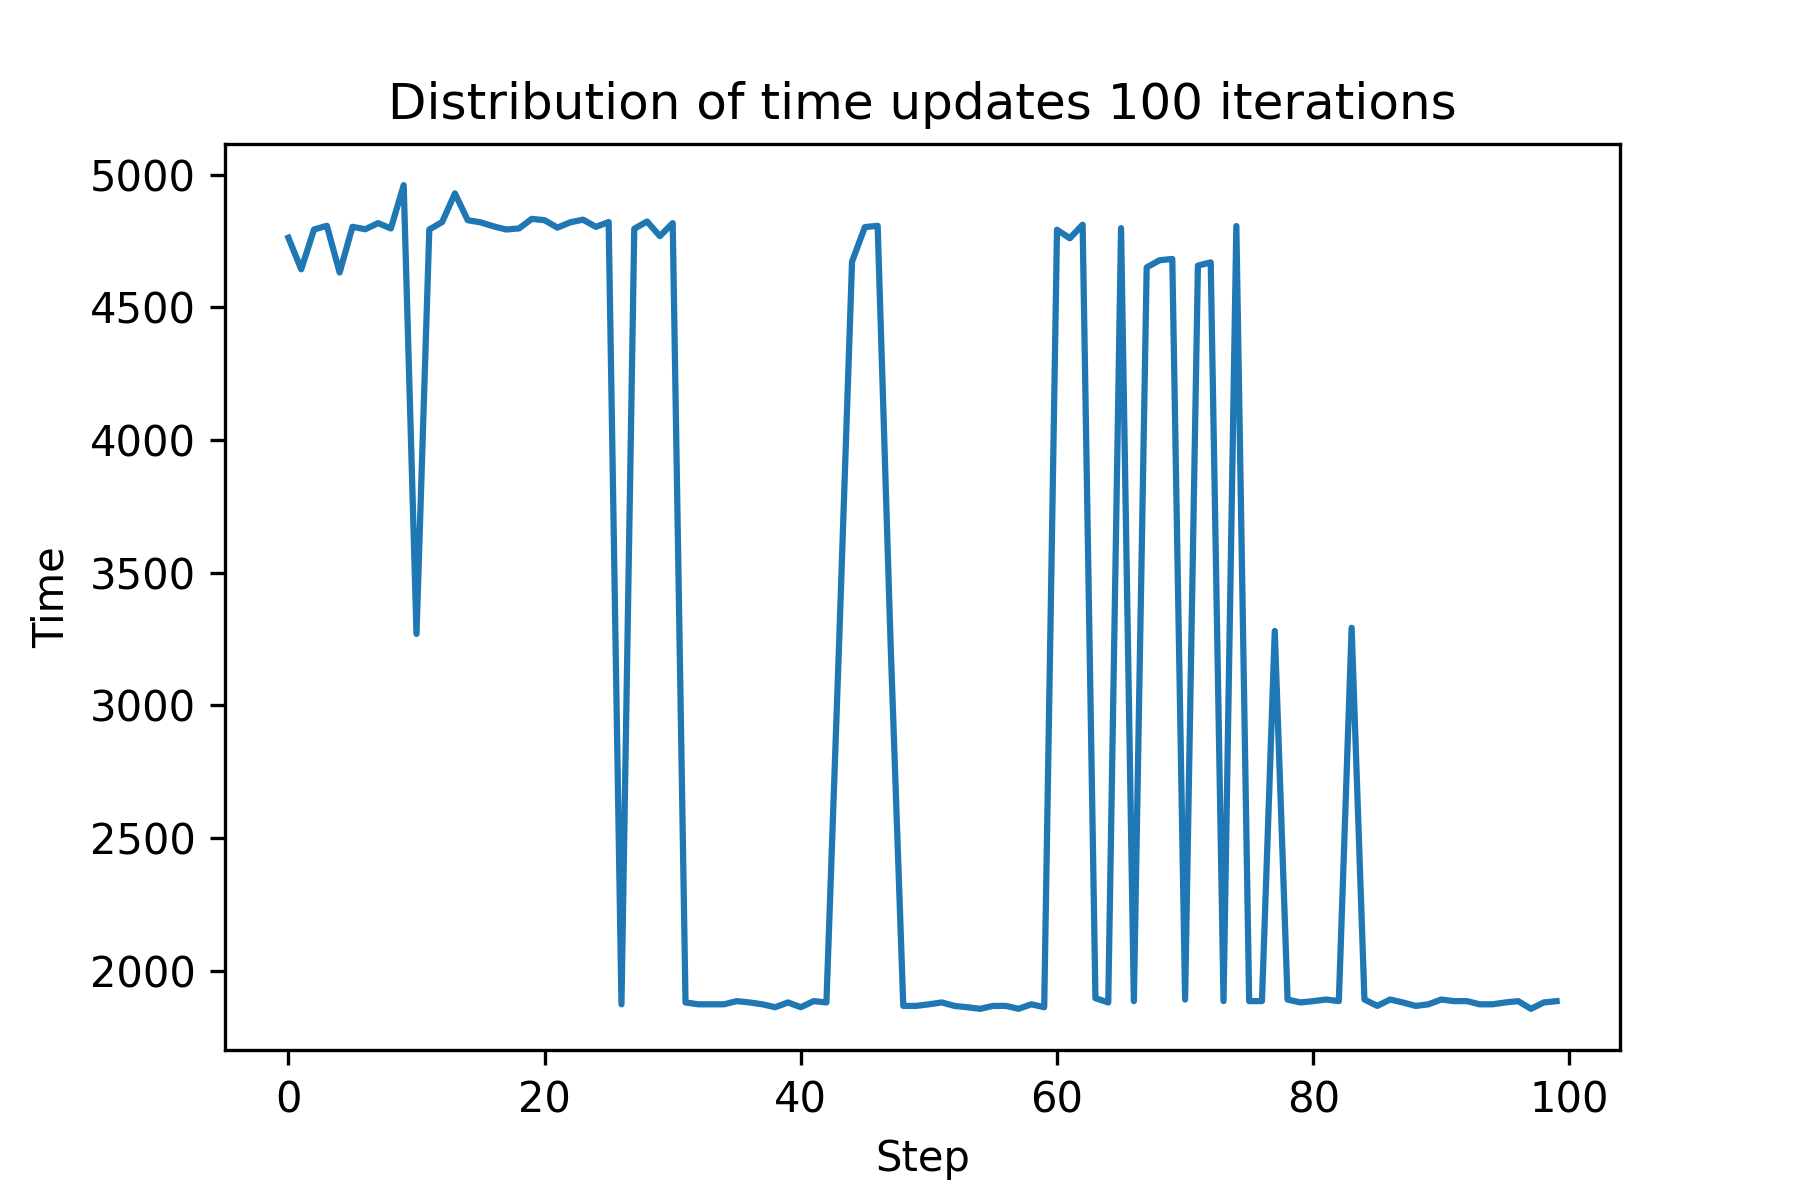
\includegraphics[width=\textwidth]{Images/plot_distribution_time_update_100.png}
         \caption{Plot of backpropagation time for 100 iterations.}
         \label{fig:time_100_iterations}
     \end{subfigure}
     \hfill
     \begin{subfigure}[b]{0.4\textwidth}
         \centering
         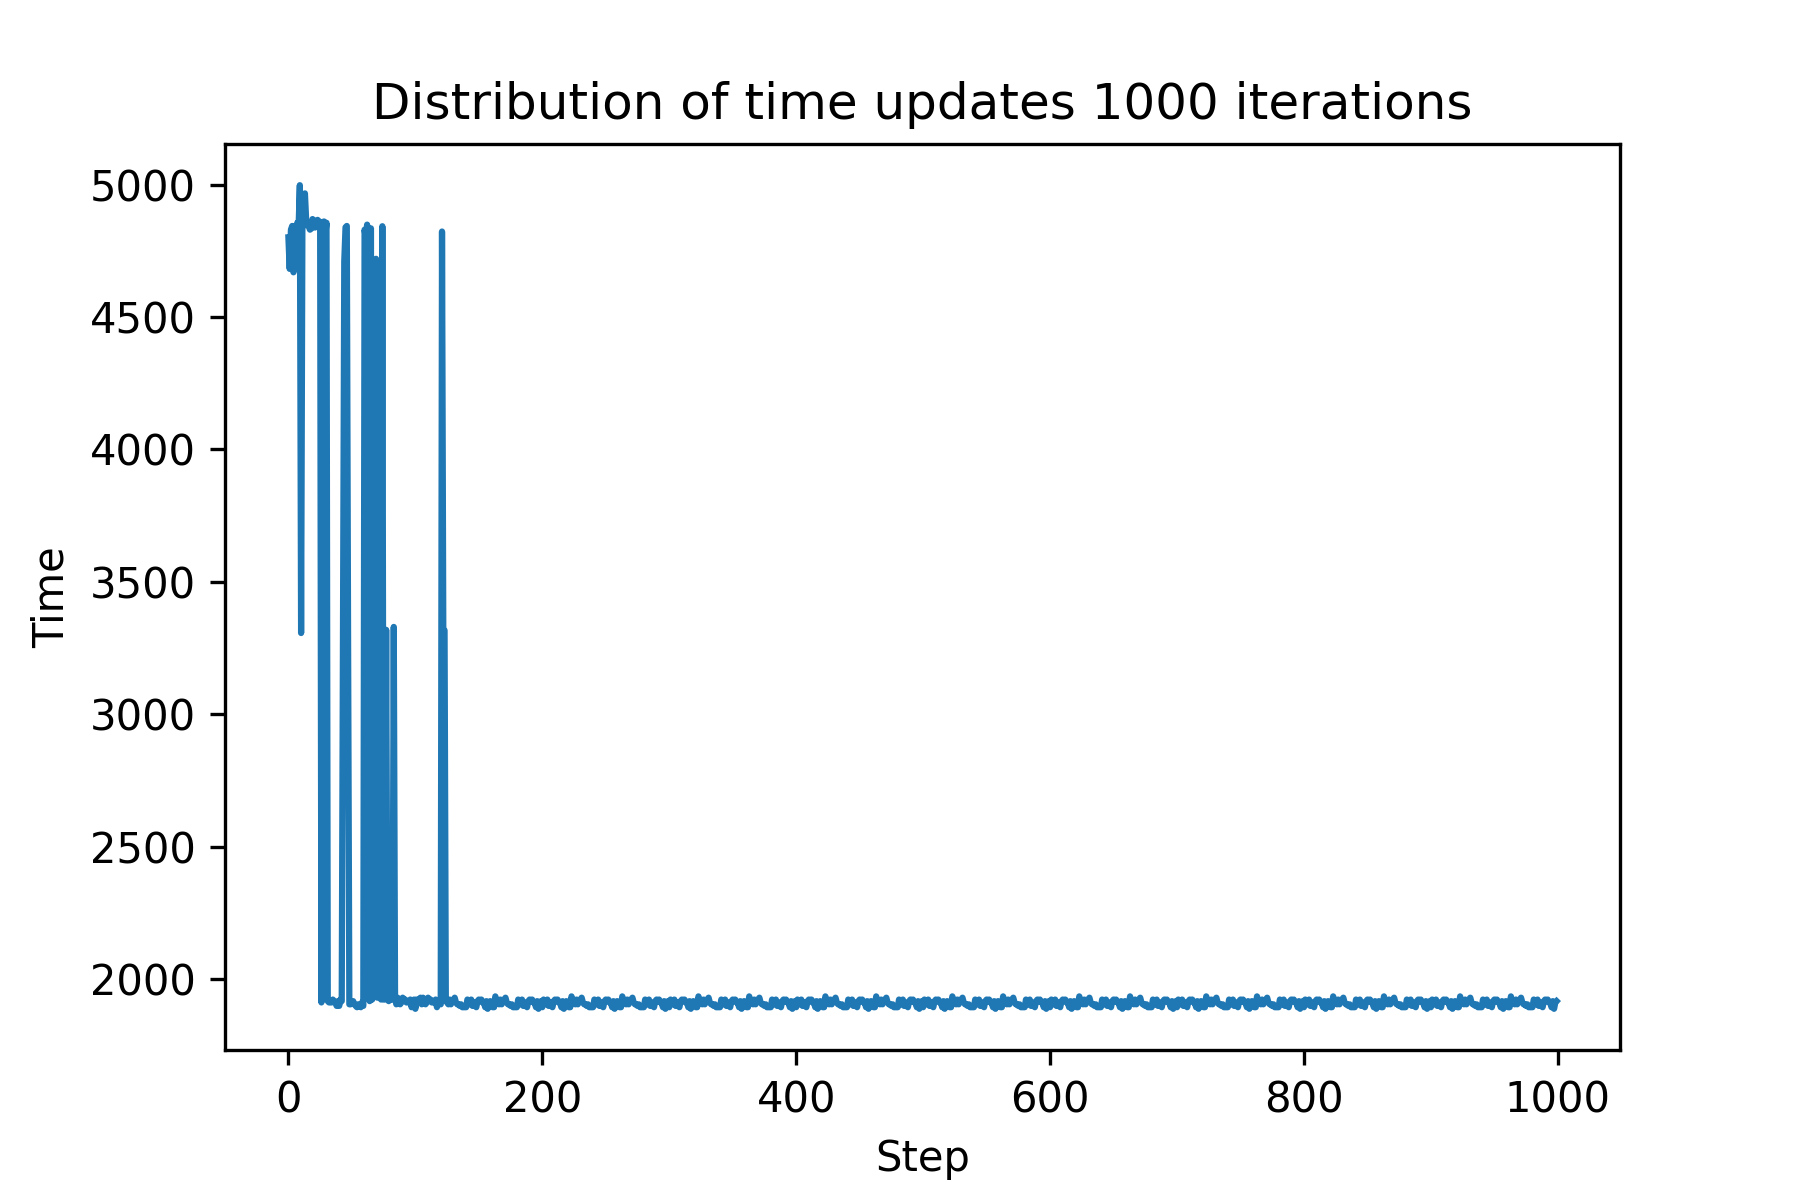
\includegraphics[width=\textwidth]{Images/plot_distribution_time_update_1000.png}
         \caption{Plot of backpropagation time for 1000 iterations.}
         \label{fig:time_1000_iterations}
     \end{subfigure}
     \hfill
        \caption{Distribution of the time that backpropagation takes at each iteration}
        \label{time_backpropagations_iterations}
\end{figure}

\singlespacing

\quad Low energy consumption is a key feature in the MCU field. Table \ref{energy_consume} contains an overview of energy consumption. This table shows the comparison between different clock sources, such as 100 MHz, 60 MHz, and 7.328 MHz. It is possible to state that the average energy consumed by the device is low. It is interesting to notice that the energy consumption at 60 MHz is lower than 100 MHz, but when the clock is reduced drastically to 7.328 MHz, the energy utilization grows exponentially. The clock source is almost fourteen times slower than the fastest, but the energy drained is nearly four times higher. Operations consume less because program execution is slower; on the other hand, the formula 
\begin{gather*}
   Energy = Power \cdot Time
\end{gather*}
\quad implies that proportionally with a longer execution time, there will be equally higher energy consumption.

\begin{figure}[!ht]
\centerline{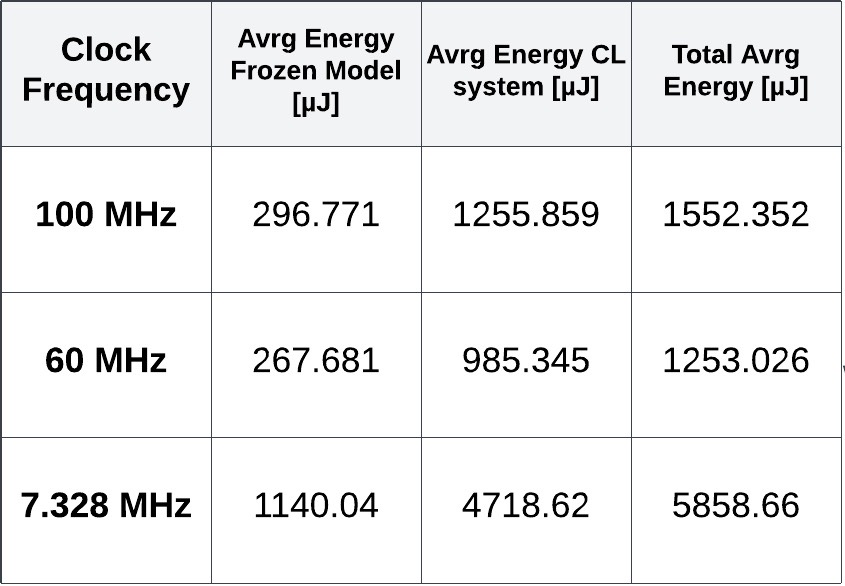
\psfig{file=Images/energy_cnn_cl.png,width=0.8\textwidth}}
\caption{Table showing the energy consumed with different clock source and by CNN and CL system.}
\label{energy_consume}
\end{figure}

\singlespacing

\quad Figure \ref{plot_accuracy} shows the model accuracy over iterations. It is possible to notice that after enough iterations, the model can recognize images more accurately. The plot serves as evidence that the algorithms are reliable and well-implemented. Furthermore, it should be highlighted that this experiment does not show significant catastrophic forgetting. After the algorithm finishes, the program computes an inference on the Mnist dataset resulting in 100\% accuracy on the right class.

\begin{figure}[!ht]
\centering
     \begin{subfigure}[b]{0.4\textwidth}
         \centering
         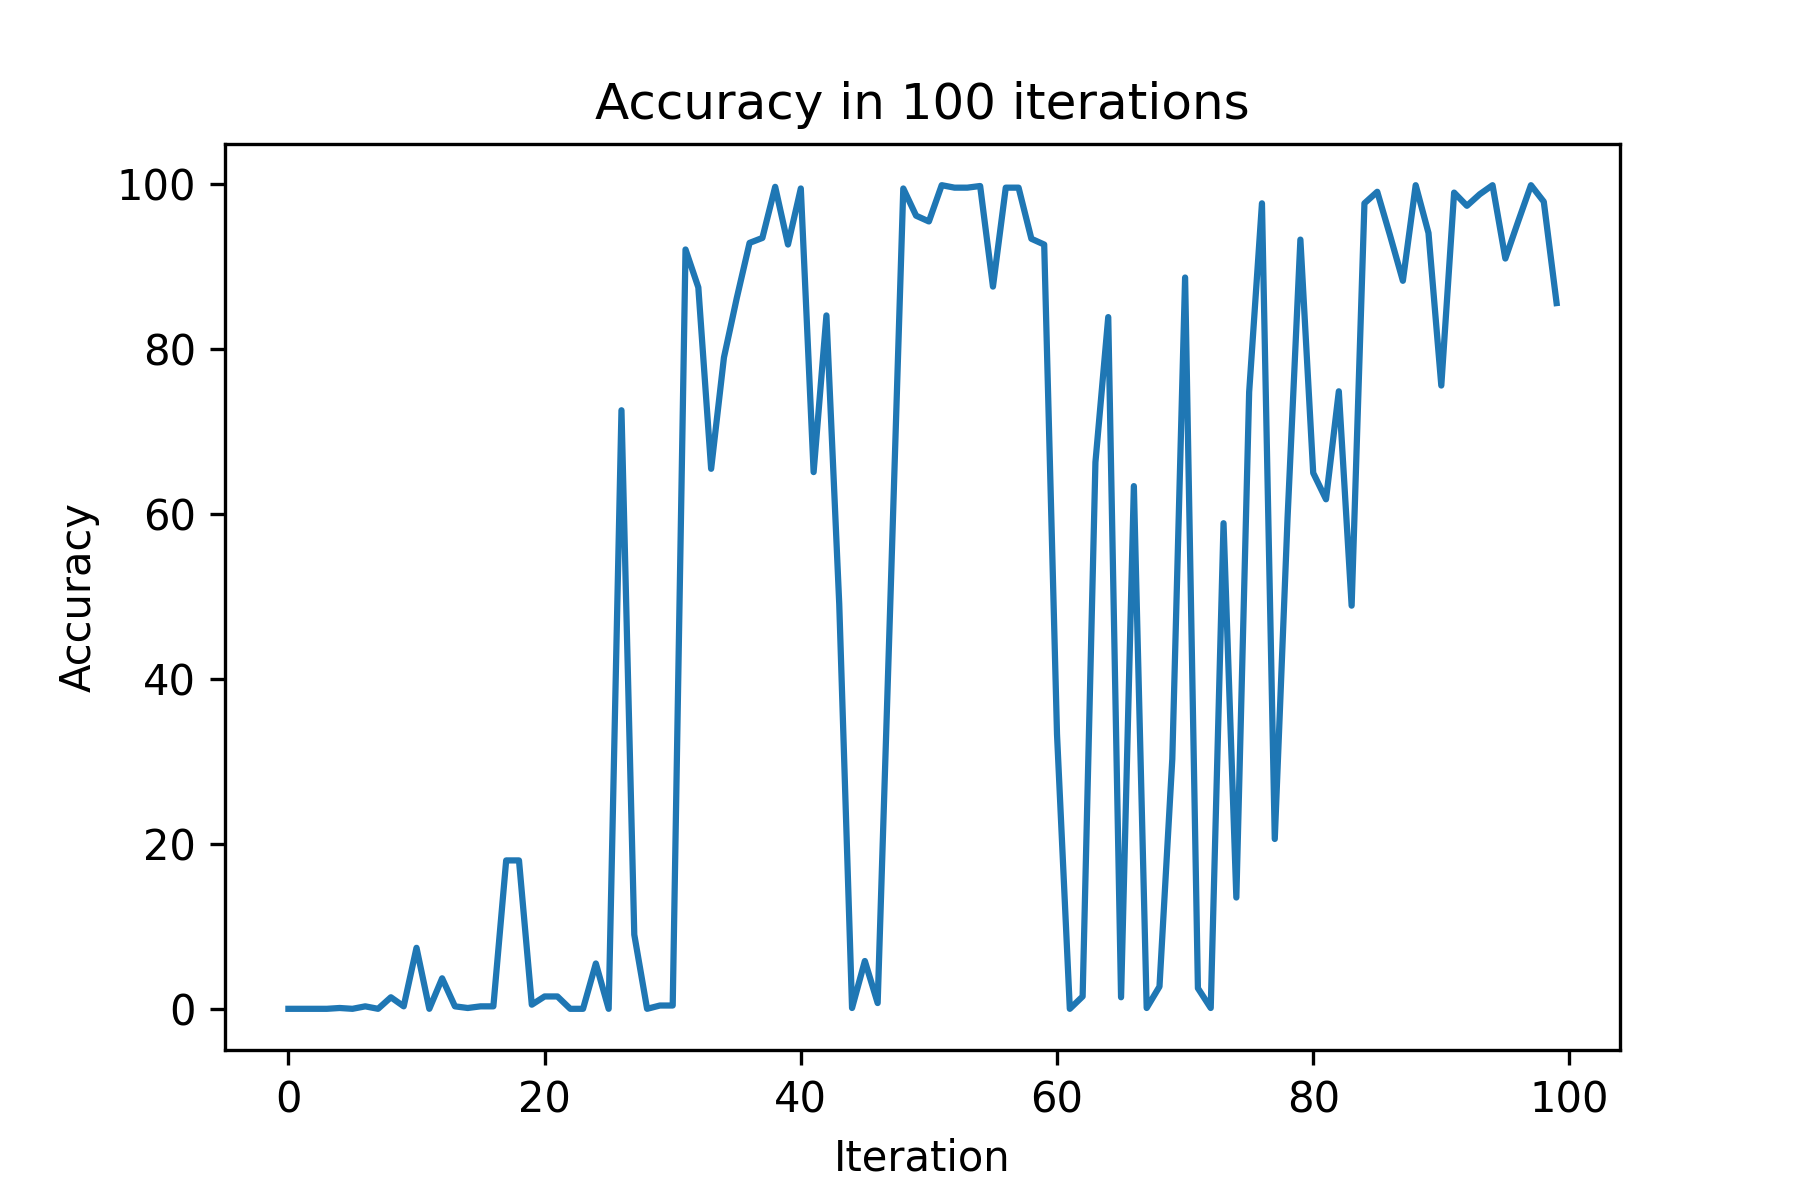
\includegraphics[width=\textwidth]{Images/plot_accuracy_100.png}
         \caption{Plot of accuracy over 100 iterations.}
         \label{fig:accuracy_100}
     \end{subfigure}
     \hfill
     \begin{subfigure}[b]{0.4\textwidth}
         \centering
         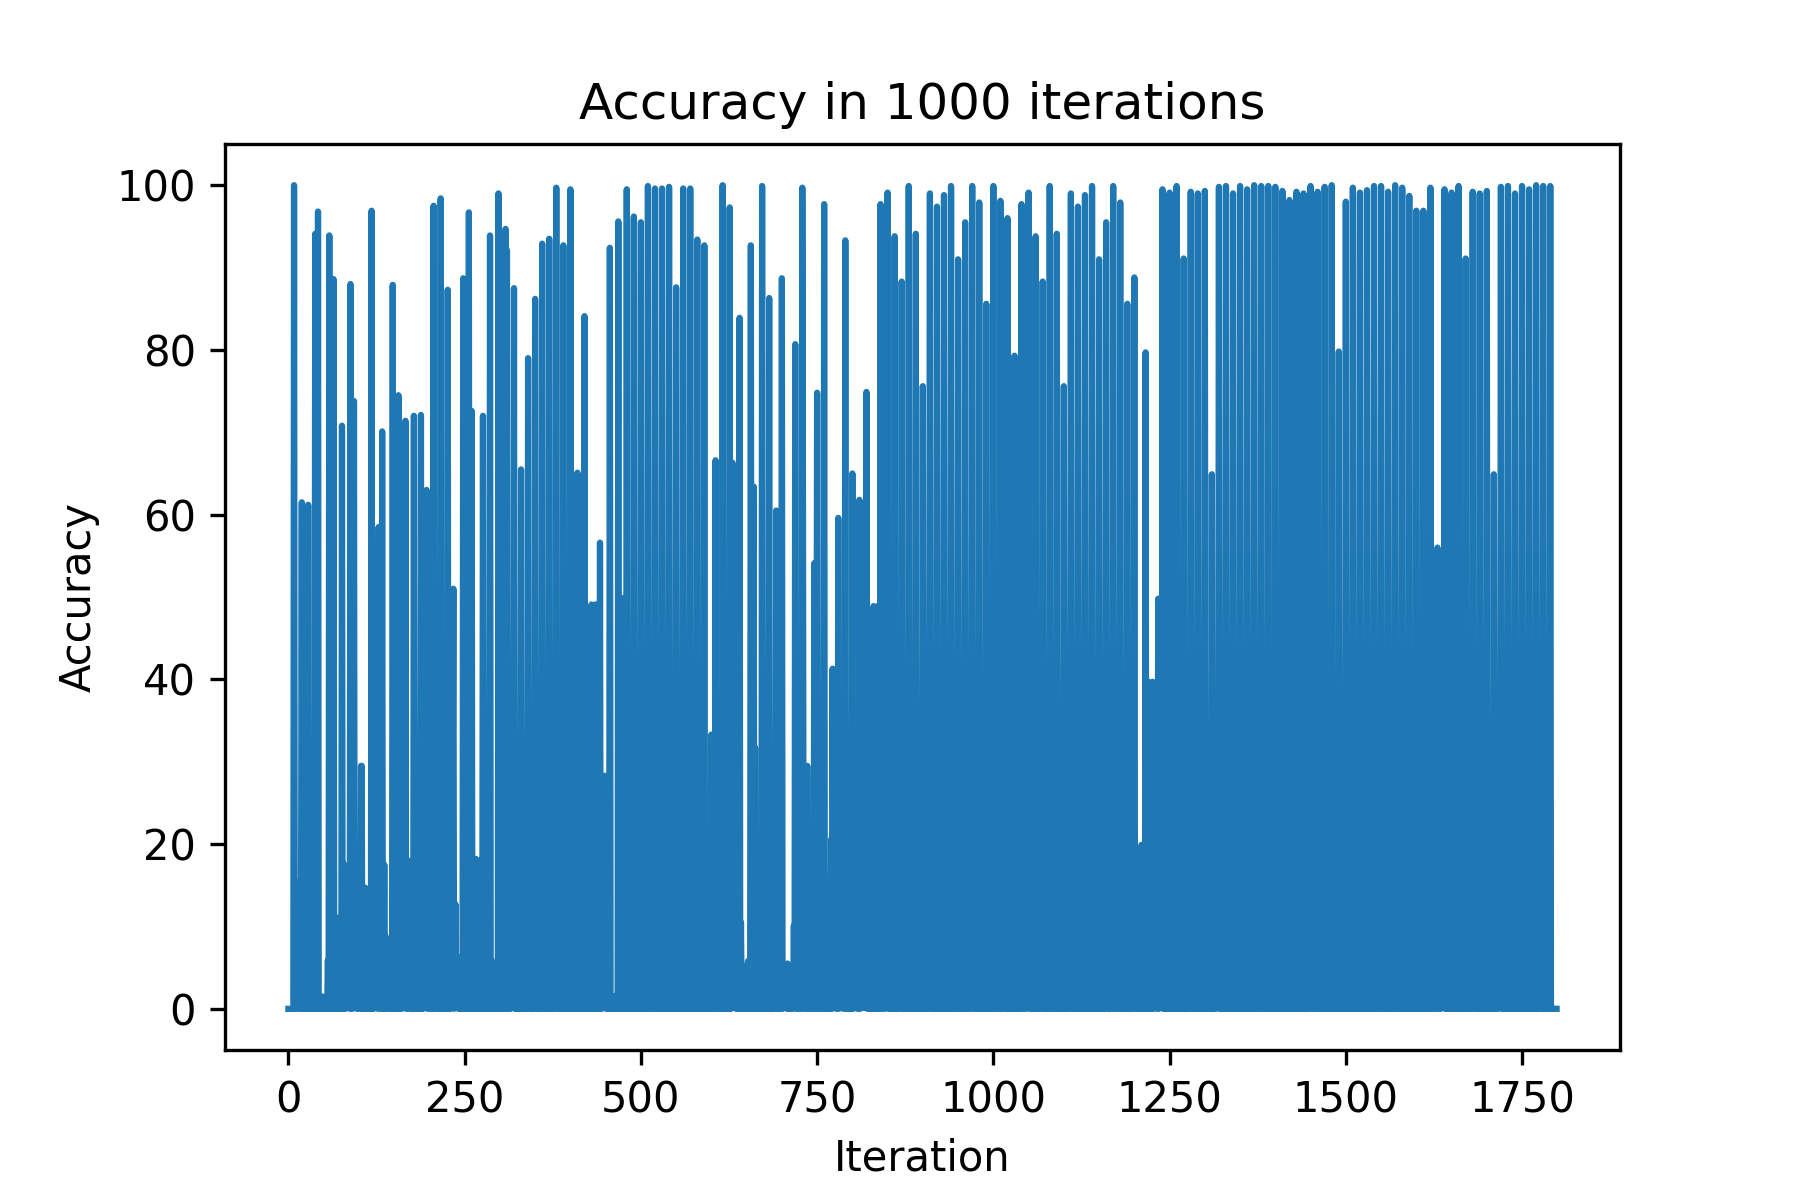
\includegraphics[width=\textwidth]{Images/plot_accuracy_1000.png}
         \caption{Plot of accuracy over 1000 iterations.}
         \label{fig:accuracy_1000}
     \end{subfigure}
     \hfill
        \caption{Plot of the percentage of accuracy.}
        \label{plot_accuracy}
\end{figure}


\clearpage
\newpage
\mbox{~}
\clearpage
\newpage
